\documentclass{beamer}
\usecolortheme{wolverine}

% math stuff
\usepackage{amsmath}
\usepackage{amsthm}
\usepackage{amssymb}
\usepackage{xcolor}

\usepackage{float}
\usepackage{subcaption}

% to insert images
\usepackage{graphicx}

% to correctly insert stressed characters
\usepackage[T1]{fontenc}
\usepackage[utf8]{inputenc}

\usepackage{multirow}

% Bibliography
% \usepackage[style=alphabetic]{biblatex}
% \usepackage[nottoc]{tocbibind}
% \usepackage{bibentry}
% \setcounter{biburllcpenalty}{9000}
% \usepackage{nameref}
% \addbibresource{slides.bib}

% to put links in table of contents
\usepackage{hyperref}
\hypersetup{colorlinks=false, %set true if you want colored links
	linktoc=all,     %set to all if you
}

\usepackage{mathtools}

% Add symbols
% \usepackage{textcomp}

% Add command for Real and Z sets
% \usepackage{dsfont}
% \newcommand{\Rset}{$\mathds{R}$}
% \newcommand{\Zset}{$\mathds{Z}$}

% Code highlighting
% \usepackage{minted}
% \usemintedstyle{perldoc}
% \setminted{
%     frame=single,
%     breaklines,
% }

% tikz figures
% \usepackage{tikzit}
% \input{style.tikzstyles}

% number rounding
\usepackage{siunitx}
\sisetup{round-mode=places,round-precision=5}

\definecolor{myyellow}{RGB}{225, 225, 0}

\title{Thesis notes}
\date{13th July}

% any code between @(...)@ is escaped back to LaTeX
% \lstset{escapeinside={@(}{)@}}

% algorithms
\usepackage[ruled,vlined]{algorithm2e}
% \newtheorem{theorem}{Theorem}

\begin{document}
\frame{\titlepage}



\begin{frame}[c]
    \frametitle{The Echo Chamber Problem}
    \textbf{Goal}: given an interaction graph $G$, find $U \subseteq V$ maximing

    \begin{equation}
        \xi (U) = \sum^{}_{C \in \hat{\mathcal{C}} } \sum^{}_{T[U] \in S_C (U)}
        (| T^{+} [U] | - | T^{-} [U] |)
    \end{equation}

    where $| T^{-} [U] |$ and $| T^{+} [U] |$ denotes the number of negative
    and positive edges induced in the subgraph, respectively.

    \bigskip

    The set of users maximing the expression is denoted as $\hat{U}$ and the
    corresponding score is $\xi(G)$
\end{frame}

\begin{frame}[c]
    \frametitle{Purity scores}
    New score for evaluating our method
    \begin{equation}
        \text{Purity}(U) = \frac{\text{\# nodes with majority label}}{|U|} 
    \end{equation}
\end{frame}

\begin{frame}[c]
    \frametitle{Evaluation algorithm}

    Evaluation algorithm for a graph $G = (V, E)$ with $\mathcal{I} $
    communities.
    \bigskip

    \begin{algorithm}[H]
	\SetAlgoLined

	\ForEach{ $i \in \mathcal{I} $ }{
		$U \leftarrow $ solve ECP on $G$ \;
		// Remove edges contributing to $\xi(U)$ \;
		$E \leftarrow E \setminus \{ e_{ij} \in E_k, T_k \in \mathcal{S}_C(U),
			C \in \mathcal{\hat{C}}\}$ \;

        $C_U \leftarrow $ components of $G[U]$ considering only positive edges\;

		$l_j \leftarrow $ majority label of users $C_j$ in $\mathcal{L}, \; \forall C_j
        \in C_U$ \;
        $P_j$ = Purity($C_j$) $\forall C_j \in C_U $
	}

	\caption{Clustering process}
	\label{alg:clustering_process}
\end{algorithm}
    
\end{frame}

\begin{frame}[c]
    \frametitle{Scores of @nytimes}

    Dataset has 80\% with one label and the remaining 20\% having another label

    \begin{figure}[H]
        \centering
        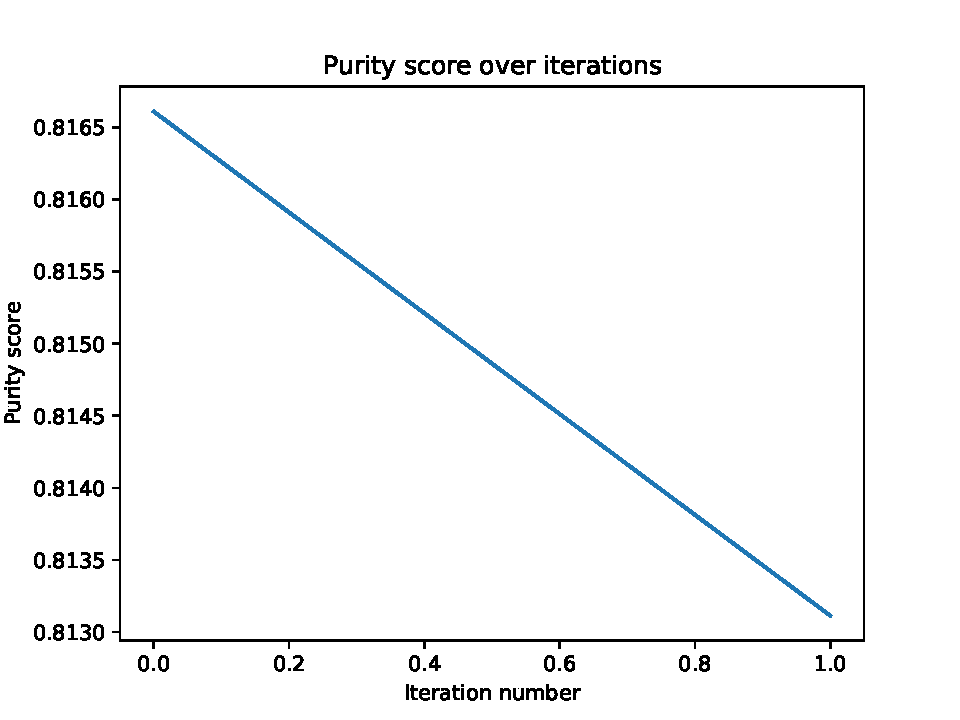
\includegraphics[width=0.8\linewidth]{./out/nytimes_baseline200/purity_iterations.pdf}
    \end{figure}
\end{frame}

\begin{frame}[c]
    \frametitle{Results analysis}
    \begin{itemize}
        \item Most of the components with scores $0.5$ or $1$ have two vertices
            \item Fraction of components with purity scores of $1$ are similar
                to the fraction of pure components if randomly sampling two
                vertices from the graph
    \end{itemize}
\end{frame}

\begin{frame}[c]
    \frametitle{Improved Twitter labeling (1)}
    Based on "Birds of a Feather Tweet Together. Bayesian Ideal Point
    Estimation Using Twitter Data" by Barberá 

    Parameters of the model
    \begin{itemize}
        \item $\phi_i$ and $\theta_j$ idealogical dimension of user $i$ and
            politician $j$. $\phi_i, \theta_j \in \mathbff{R}$  
        \item $\alpha _i$ political interest of user $i$
        \item $\beta _j$ popularity of politician $j$
    \end{itemize}

\end{frame}

\begin{frame}[c]
    \frametitle{Improved Twitter labeling (2)}
    \begin{enumerate}
        \item Obtain set of users $O$ as in the paper
            \begin{itemize}
                \item Start from politicians $P$ and mine followers
                \item Exclude inactive users and bots
            \end{itemize}
        \item Consider subset of $O$ following at least $10$ politicians
        \item Use them to estimate parameters indexed by $j$ \pause
        \item {\color{blue} Use these parameters to fit parameters of users
            in $U$
        \item For each user $u \in U$, $label_u = \text{democrat}$ if 
            \begin{equation}
                label_u = \begin{cases}
                    democrat, &\text{ if }\phi_u < 0\\
                    republican, &\text{ otherwise}.
                \end{cases}
            \end{equation}}
            (during parameters initialization, democrats $\theta _j = -1$ and republicans $\theta_j = 1$).
    \end{enumerate}
\end{frame}

\begin{frame}[c]
    \frametitle{Improved Twitter labeling (3)}
    Possible variant: take into account also political involvement of user
    $\alpha _i$ and exclude users with low involvement.
\end{frame}

\end{document}
